\chapter{Transistor}
\label{v:18}

In diesem Versuch soll die grundlegende Funktion als Leistungsverstärker eines Transistors studiert werden.

%------------------------------------------------
\section{Stichworte}
%------------------------------------------------

Halbleiter; $pn$-Übergang; Wirkungsweise eines Transistors; Emitterschaltung; Transistorkennlinie; Transistor als Verstärker.
%
%------------------------------------------------
\section{Literatur}
%------------------------------------------------

Gehrtsen, Kapitel 14.4.1-3
%
%------------------------------------------------
\section{Anwendungsbeispiele}
%------------------------------------------------

Transistoren gehören zu den wichtigsten elektronischen Bauelementen. Sie werden zum Verstärken und Schalten elektrischer Signale verwendet. Meist bestehen sie aus drei Zonen von halbleitendem Material, das verschieden dotiert ist (p- oder n-leitend). Diese Dreiteilung erinnert noch an ihre Vorläufer, die Trioden. Daher existieren in der Nomenklatur auch viele Ähnlichkeiten. Diese Vakuum-Röhren, deren Funktion man meist schneller begreift, erhalten ihre beweglichen Ladungsträger (Elektronen) aus einem Heizdraht, sie werden auf eine positiven Elektrode hin beschleunigt und können durch ein dazwischen liegendes Gitter abgebremst oder durchgelassen werden. Im Transistor bewegen sich die (negativen oder positiven) Ladungsträger durch Festkörpergrenzflächen, wieder geregelt durch Ladungen, die von außen beeinflusst werden.\\
Eine Vielzahl von Transistoren oder anderen Bauelementen (z.B. Widerstände) können in einem einzigen Fertigungsprozess auf einem einkristallinen Siliziumplättchen (Chip) hergestellt werden. Vor einigen Jahren überschlugen sich die Computer-Chip Hersteller noch mit Angaben, wie viel Tausend Transistoren auf einem Quadratzentimeter Platz hätten. Heute ist es um diese Zahlen still geworden, weil sie so astronomisch groß geworden sind, dass man sie nur noch in Zehnerpotenzen angeben kann, die dann aber doch keiner mehr begreift.\\
Es lohnt sich, sich mit diesem, zugegebenermaßen komplizierten, Bauelement näher zu beschäftigen, das in allen Regelungen und Computern steckt und schon unsichtbar klein geworden ist und unser Leben im letzten Jahrhundert so grundlegend geändert hat.

%------------------------------------------------
\section{Theoretischer Hintergrund}
%------------------------------------------------

\subsection{Der (unbelastete) Spannungsteiler}

	\begin{figure}[h!]
		\centering
		\begin{circuitikz}
			\begin{scope}[xshift=0cm]
				\draw (2.5,2)
					to [R, i<_=$I$, l=$R_1$](0,2) 
					to [V_=$U_o$] (0,0) 
					to [short] (2.5,0) coordinate (B)
					to [R, l=$R_2$] (2.5,2) coordinate (A);
				\draw (A) to [short, *-o] ++(0.5,0) coordinate (A1);
				\draw (A1) node [anchor=south] {$A$};
				\draw (B) to [short, *-o] ++(0.5,0) coordinate (B1);
				\draw (B1) node [anchor=north] {$B$};
				\draw (B1) to [open, v=$U_{AB}$] (A1);
			\end{scope}
		\end{circuitikz}
		\caption{Spannungsteiler}
		\label{fig:spannungsteiler}
	\end{figure}
Schaltet man, wie in Abbildung \ref{fig:spannungsteiler}, zwei Widerstände $R_1$ und $R_2$ hintereinander (in Serie), so fließt durch beide Widerstände derselbe Strom $I$. Die Spannung $U_0$, die die Spannungsquelle zur Verfügung stellt, fällt über beide Widerstände ab nach dem Ohm'schen Gesetz $U_0 = R\cdot I = \left( R_1 + R_2\right)\cdot I$. Über jeden einzelnen Widerstand fällt also nur ein Teil der gesamten Spannung ab: $U_0 = U_1 + U_2 = R_1\cdot I + R_2\cdot I$.\\
Diese \textit{Spannungsteiler} genannte Schaltung wird häufig benutzt, wenn man an einen Verbraucher nicht die ganze Spannung $U_0$ anlegen will oder darf. Stattdessen schließt man den Verbraucher zum Beispiel an die Klemmen $A$ und $B$ an, so dass an ihm die Spannung $U_{AB}$ liegt. Wie groß diese Spannung ist, kann man nun aus den obigen Gleichungen berechnen. Diese folgen aus den sogenannten Kirchhoff'schen Gesetzen, die Sie in Versuch \ref{v:13} genauer kennenlernen.\\
Für den Fall, dass der Verbraucher nicht viel Strom zieht, die Spannung $U_{AB}$ wie folgt berechnet werden kann:
\begin{equation}
	U_{AB} = U_0\cdot\frac{R_2}{R_1 + R_2}
\end{equation}
In diesem Versuch werden Sie die Spannungsteilerschaltung benutzen, um mehrere verschiedene, variable Spannungen an die Anschlüsse des Transistors anzulegen, obwohl nur ein einziges Netzgerät zur Verfügung steht.

\subsection{Der Bipolartransistor}

Werden zwei Elektronen-Halbleiter (n-Leiter) durch eine Schicht eines Löcher-Halbleiters (p-Leiter) getrennt, deren Schichtdicke in der Größenordnung der Ausdehnung des an den Grenzflächen aufgebauten elektrischen Feldes liegt 
($10^{-5}$ m), so kann ein Teil der Elektronen durch die Schicht hindurchtreten. Das Ausmaß des durchtretenden Teiles hängt von der Stärke des elektrischen Feldes ab. Dieses Feld kann von aussen durch Anlegen einer elektrischen Spannung an die dünne Schicht beeinflusst werden. Damit wird der Durchtritt der Elektronen steuerbar!\\
Der Strom $I_C$, der durch den Transistor fließt, lässt sich durch den Basisstrom $I_B$ steuern. Die Verstärkerwirkung des Transistors beruht darauf, dass im Sättigungsbereich der Transistorkennlinie kleine Änderungen des Basisstroms große Änderungen des Kollektorstroms bewirken.\\

\noindent
Die dünne Schicht, Basis $B$ genannt, übernimmt damit ähnliche Funktion wie das Gitter der Triodenröhre. Der an die Basis Elektronen abgebende n-Leiter heißt Emitter $E$. Er hat eine ähnliche Funktion wie die Kathode in der Triodenröhre. Der Elektronen aufnehmende Teil heißt Kollektor $C$ und entspricht der Anode in der Triodenröhre.\\
Das beschriebene System ist ein npn-Transistor. Mit p werden die positiven Ladungsträger (Löcher) der Basis $B$, symbolisiert, während n für die negativen Ladungsträger (Elektronen) im Emitter $E$ und im Kollektor $C$ steht. Ein pnp-Transistor funktioniert analog, aber mit umgekehrten Vorzeichen der Ladungen, Ströme und Spannungen.\\

\noindent
Dieser Transistor hat zwei pn-Übergänge und man kann ihn sich stark vereinfacht als zwei entgegengesetzt geschaltete Dioden vorstellen (siehe Abbildung).\\
In der sog. Emitterschaltung (s. Versuchsaufbau) ist die E-B-Diode in Durchlassrichtung geschaltet, d.h. Elektronen können von E nach B gelangen und es fließt ein (kleiner) Basisstrom. Der Kollektor liegt gegenüber der Basis auf positivem Potential, also ist die C-B-Diode in Sperrrichtung geschaltet. Der Strom $I_C$ ist der Sperrstrom der C-B-Diode und ist abhängig von der Anzahl der Elektronen in der p-leitenden Basis (s. Versuch \ref{v:17}). Da die B-E-Diode in Durchlassrichtung geschaltet ist, hängt die Elektronenkonzentration in der Basis von der äußeren Spannung $U_{BE}$ bzw. vom Basisstrom $I_B$ ab. Dadurch ist der Kollektorstrom $I_C$ eine Funktion sowohl von der äußeren Spannung $U_{EC}$ zwischen Emitter und Kollektor als auch vom Basisstrom $I_B$: $I_C = I_C (U_{EC} , I_B)$\\

\noindent
Sehr stark vereinfachend kann man sich einen Transistor in dieser Beschaltung, bei konstanter Kollektor-Emitter-Spannung $U_CE$, also ähnlich wie eine Stromquelle vorstellen, deren Ausgangsstrom durch die zwischen Basis und Emitter angelegte Spannung $U_{BE}$ eingestellt werden kann.\\
Eine der angenehmen Eigenschaften der Bipolartransistoren ist, dass der Kollektorstrom $I_C$ linear vom Basisstrom abhängt:
\begin{equation}
	I_C = \beta\cdot I_B\; .
\end{equation}
Den Proportionalitätsfaktor $\beta$ bezeichnet man als Stromverstärkungsfaktor des Transistors. Dieser hängt vom genauen Aufbau des Transistors ab, also der Breite der Basiszone und den Ladungsträgerkonzentrationen in den verschieden dotierten Bereichen, und kann somit von Transistor zu Transistor signifikant unterschiedlich sein.

%------------------------------------------------
\section{Fragen zur Vorbereitung}
%------------------------------------------------

\begin{enumerate}
	%
	%\item Was soll heute im Praktikum gemessen werden? Warum?
	%
	\item Was ist eine Spannungsteilerschaltung?
	%
	\item Wozu kann ein Transistor benutzt werden? Nennen Sie Beispiele!
	%
	\item Aus welchen Halbleitern wird ein Transistor aufgebaut?
	%
	\item Wie sind die Spannungen an den einzelnen Schichten bei der im Versuch verwendeten Emitterschaltung geschaltet?
	%
	\item Was versteht man unter Basis, Emitter und Kollektor?
	%
	\item Wie funktioniert ein Transistor in Emitterschaltung? Welche entscheidende Rolle spielt dabei die Basis?
	%
	\item Welcher Strom kann mit dem Basisstrom geregelt werden?
	%
	\item Wie sehen die Ausgangskennlinien eines Transistors in Emitterschaltung aus? Von welchem Parameter hängen die Kennlinien ab?
	%
	\item Was vergleicht man mit dem Verstärkungsfaktor eines Transistors? Wie berechnet sich der Verstärkungsfaktor des Transistors?
	%
\end{enumerate}

%------------------------------------------------
\section{Durchführung} 
%------------------------------------------------

\begin{figure}[h]
	\centering
		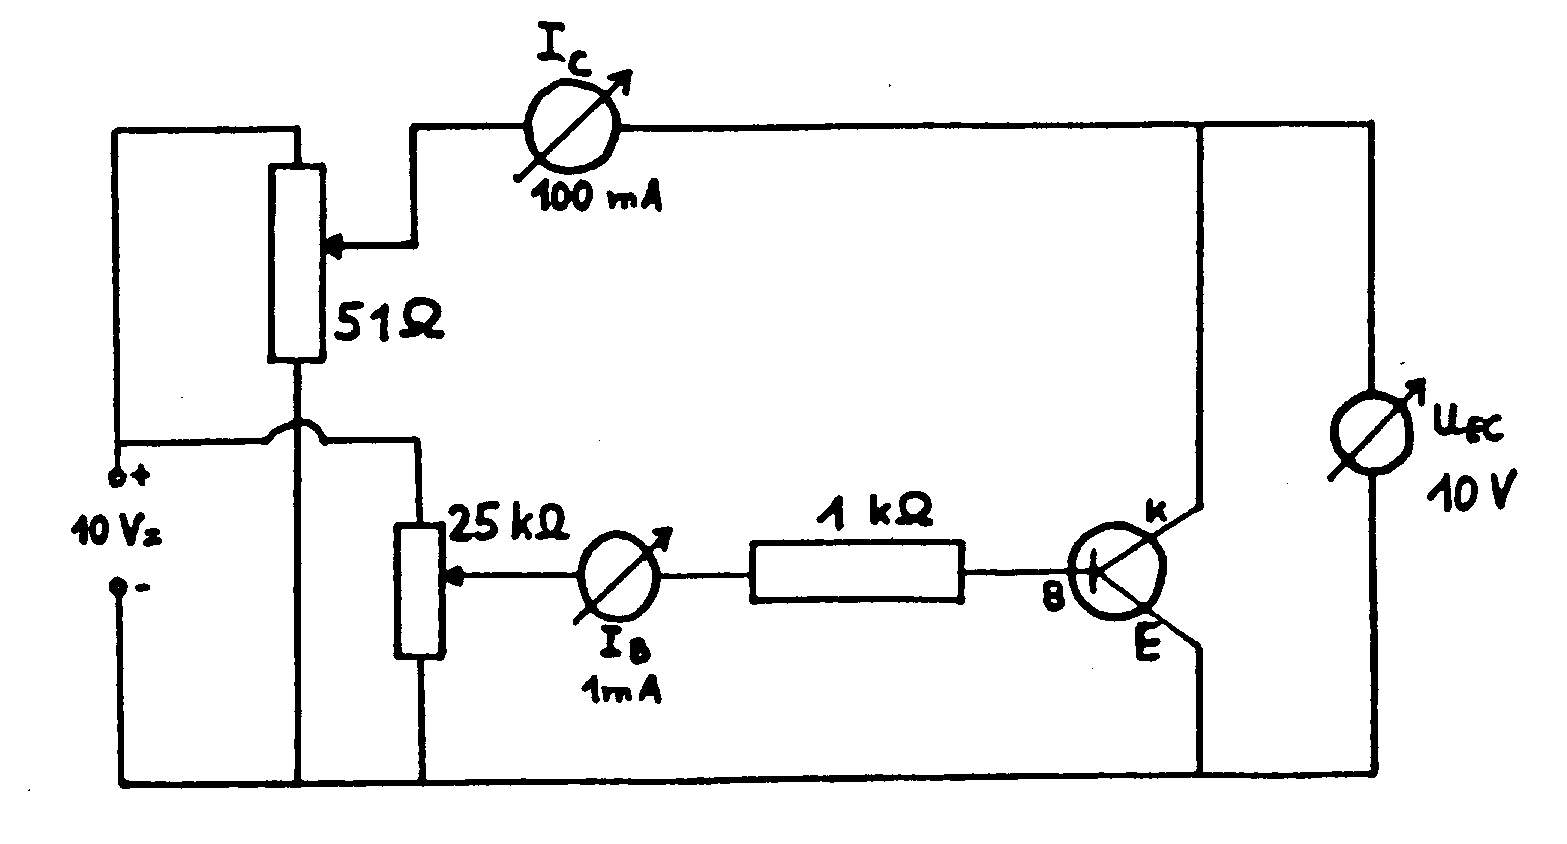
\includegraphics[width=0.75\textwidth]{Abbildungen/BILD23.JPG}
	\label{fig:BILD23}
\end{figure}

\begin{enumerate}
	%
	\item Bauen Sie die Schaltung gemäß des Schaltplanes auf und lassen sie diese vom Assistenten kontrollieren.
	%
	\item Stellen sie einen Basisstrom $I_B$ von 0.2\,mA ein. Messen Sie den Kollektorstrom $I_C$ in Abhängigkeit von der Spannung $U_{EC}$ ($U_{EC}$ = 0, 0.1, 0.2, 0.3, 0.4, 0.5\,V anschließend 1\,V, 2\,V, 3\,V, ..., 10\,V).
		Regeln Sie dabei den Basisstrom $I_B$ immer nach.
	%
	\item Wiederholen Sie die Messung für verschiedene Basisströme $I_B$ = 0.3, 0.4, 0.5\,mA.
	%
\end{enumerate}

%------------------------------------------------
\section{Auswertung} 
%------------------------------------------------

\begin{enumerate}
	%
	\item Tragen Sie das Ausgangskennlinienfeld $I_C (U_E)$ für die vier Basisströme auf.
	%
	\item Entnehmen Sie aus Ihren Messreihen zu jedem Basisstrom $I_B$ die Werte des Kollektorstoms $I_C$ bei einer Spannung $U_{EC}$ = 8\,V. Tragen Sie diese auf und bestimmen sie graphisch den Verstärkungsfaktor $\beta$ mit Fehler.
\end{enumerate}